\chapter{Organization and Management}
\label{v1ch:org-mgmt}

%%%%%%%%%%%%%%%%%%%%%%%%%%%%%%%%%%%%%%%%%%%%%%%%%%%%%%%%%%%%%%
\section{Overview}

To accommodate a variety of international funding model constraints, LBNF and DUNE are organized as separate projects. As mentioned in the Introduction, the LBNF Project is responsible for design and construction of the conventional facilities, beamlines, and cryogenic infrastructure needed to support the experiment.  The DUNE Project is responsible for the construction and commissioning of the detectors used to pursue the scientific program.  LBNF is organized as a DOE/Fermilab project incorporating international partners.   DUNE is an international project organized by the DUNE Collaboration with appropriate oversight from stakeholders including the DOE.

%%%%%%%%%%%%%%%%%%%%%%%%%%%%%%%%%%%%%%%%%%%%%%%%%%%%%%%%%%%%%%
\section{LBNF}

%%%%%%%%%%%%%%%%%%%%%%%%%%%%%%%
\subsection{Project Structure and Responsibilities}

The LBNF Project is charged by Fermilab and DOE to design and construct the conventional and technical facilities needed to support the DUNE Collaboration.  LBNF works in close coordination with DUNE to ensure that the scientific requirements of the program are satisfied through the mechanisms described in Section~\ref{sec:lbnf-dune-interface}. LBNF also works closely with SURF management to coordinate the design and construction of the underground facilities required for the DUNE far detector. 

LBNF consists of two major L2 subprojects coordinated through a central Project Office located at Fermilab: Far Site Facilities and Near Site Facilities. Each L2 Project incorporates several large L3 subprojects as detailed in the WBS structure presented in Figure~\ref{fig:lbnf-wbs}.

The Project team consists of members from Fermilab, CERN, SDSTA, and BNL.  The team, including members of the Project Office as well as the L2 and L3 managers for the individual subprojects, is assembled by the Project Director. The Project team to WBS Level~3 of the WBS is shown in Figure~\ref{fig:lbnf-org}. 
Line management for environment, safety and health, and quality assurance flows through the Project Director. 


Through their delegated authority and in consultation with major stakeholders, the L2 Project Managers determine which of their lower-tier managers will be Control Account Managers (CAMs) for the Project WBS. L2 and L3 Project Managers are directly responsible for generating and maintaining the cost estimate, schedule, and resource requirements for their subprojects and for meeting the goals of their subprojects within the accepted baseline cost and schedule. 

\begin{cdrfigure}[LBNF Work Breakdown Structure to WBS Level 3]{lbnf-wbs}{LBNF Work Breakdown Structure to WBS Level 3}
  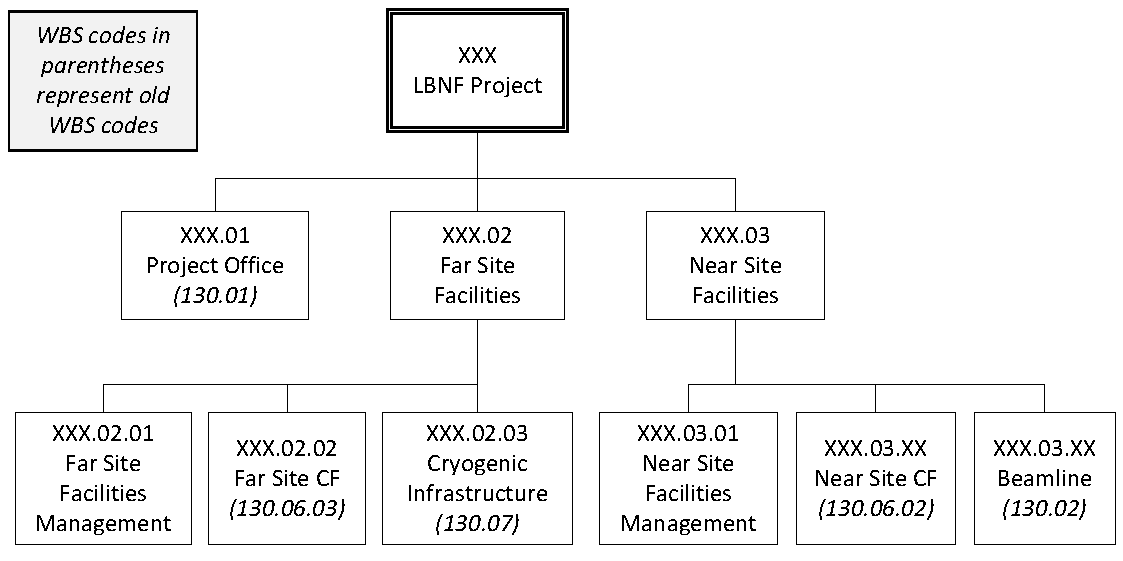
\includegraphics[width=0.8\textwidth]{lbnf-wbs-l3-nonames}
\end{cdrfigure}

The design and construction of LBNF is supported by other laboratories and consultants/contractors that provide scientific, engineering, and technical expertise. A full description of LBNF Project Management is contained within the LBNF Project Management Plan. \fixme{[ref]}

\begin{cdrfigure}[LBNF Organization]{lbnf-org}{LBNF Organization}
  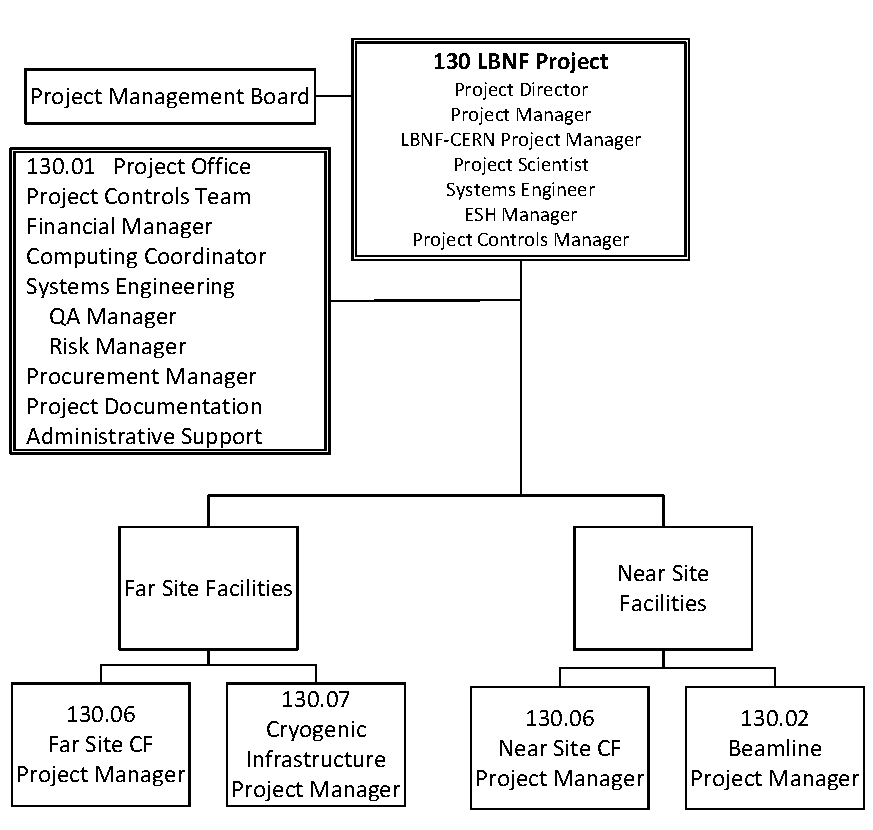
\includegraphics[width=0.8\textwidth]{lbnf-org}
\end{cdrfigure}


%%%%%%%%%%%%%%%%%%%%%%%%%%%%%%%
%%\subsection{Fermilab}

%%\fixme{Some intro text about how Fermilab is the Near Site...}

%%%%%%%%%%%%%%%%%%%%%%%%%%%%%%%
%\subsection{South Dakota Science and Technology Authority and SURF}
\subsection{SDSTA and SURF}

LBNF plans to construct facilities at SURF to house the DUNE far detector. SURF is owned by the state of South Dakota and managed by the South Dakota Science and Technology Authority (SDSTA). 

Current SURF activities include operations necessary for allowing safe access to the 4850L of the mine, which houses the existing and under-development science experiments. The DOE is presently funding SDSTA ongoing operations through Lawrence Berkeley National Laboratory (LBNL) and its SURF Operations Office through FY16; this is expected to change to funding through Fermilab starting in FY17. 

The LBNF Far Site Facilities Manager is also an employee of SDSTA and is contracted to Fermilab to provide management and coordination of the Far Site Conventional Facilities (CF) and Cryogenics Infrastructure subprojects. LBNF contracts directly with SDSTA for the design of the required CF at SURF; whereas the actual construction of the CF will be directly contracted from Fermilab. Coordination between SDSTA and the LBNF Project is necessary to ensure efficient operations at SURF. This will be facilitated via an agreement being developed between SDSTA and Fermilab regarding the LBNF Project \fixme{[new reference]} that defines responsibilities and methods for working jointly on LBNF Project design and construction. A separate agreement will be written for LBNF Operations. 

%%%%%%%%%%%%%%%%%%%%%%%%%%%%%%%
\subsection{CERN}

The European Organization for Nuclear Research (CERN) is expected to significantly contribute to LBNF with technical components , required to support the deployment of the DUNE detectors and of the neutrino beamline. 
%As a key partner in the Cryogenics Infrastructure subproject, CERN will provide engineering and technical support for the design and production of specific components and coordinate with others in LBNF on the installation of the identified deliverables. CERN engineers and scientists will participate in the LBNF Project as assigned managers for the CERN contributions.
%%as outlined in the sections below. 
%Details of the agreements with CERN will be contained in [name the agreements here]. \fixme{[name the agreements here]}.  

%%%%%%%%%%%%%%%%%%%%%%%%%%%%%%%
\subsection{Coordination within LBNF}

The LBNF Project organization is headed by the LBNF Project Director who is also the Fermilab Deputy Director for LBNF and reports directly to the Fermilab Director. 
Within Fermilab's organization, two new divisions are being created to execute the Far Site Facilities and Near Site Facilities subprojects. The heads of these divisions will report to the LBNF Project Manager. 
Any personnel working more than half-time on these subprojects would typically be expected to become a member of one of these divisions, while other contributors will likely be matrixed in part-time roles from other Fermilab Divisions.  The heads of the other Fermilab Divisions work with the L1 and L2 project managers to supply the needed resources on an annual basis.  The management structure described above is currently being transitioned into and will not be fully in place until the Fall of 2015.  

The LBNF WBS defines the scope of the work. All changes to the WBS must be approved by the LBNF Project Manager prior to implementation. At the time of CD-1-Refresh, the LBNF WBS is in transition. Both the current and the post CD-1-R WBS is shown in Figure~\ref{fig:lbnf-wbs} to demonstrate how the scope will map from one WBS to the other. 

SDSTA assigns engineers and others as required to work on specific tasks required for the LBNF Project at the SURF site. This is listed in the resource-loaded schedule as contracted work from Fermilab for Far Site CF activities. 

CERN and Fermilab are developing a common cryogenics team to design and produce the Cryogenics Infrastructure subproject deliverables for the far site. CERN provides engineers and other staff as needed to complete their agreed-upon deliverables.  

\fixme{Something about ``LBNF has formed several management groups with responsibilities as described below.''}

\textbf{Project Management Board:} LBNF uses a Project Management Board to provide formal advice to the Project Director on matters of importance to the LBNF Project as a whole. Such matters include (but are not limited to) those that:
\begin{itemize}
\item have significant technical, cost, or schedule impact on the Project
\item have impacts on more than one L2 subproject
\item affect the management systems for the Project
\item have impacts on or result from changes to other Projects on which LBNF is dependent
\item result from external reviews or reviews called by the Project Director
\end{itemize}
The Management Board serves as the
\begin{itemize}
\item LBNF Change Control Board, as described in the Configuration Management Plan \fixme{[ref]}
\item Risk Management Board, as described in the Fermilab Risk Management Plan  \fixme{[ref]}
\end{itemize}

\textbf{Beamline Technical Board:} The role of the LBNF Beamline Technical Board (TB) is to provide recommendations and advice to the Beamline Project Manager on important technical decisions that affect the design and construction of the Beamline. The members of the Technical Board must have knowledge of the Project objectives and priorities in order to perform this function. The Beamline Project Manager chairs the Beamline TB. The Beamline Project Engineer is the Scientific Secretary of the Board and co-chairs the Beamline TB as needed. 

\textbf{FSCF Neutrino Cavity Advisory Board:} The Far Site CF (FSCF) Project has engaged three international experts in hard rock underground construction to advise it periodically through the design and construction process regarding excavation at SURF. The Board meets at the request of the FSCF-PM, generally on site to discuss specific technical issues. The Board produces a report with its findings and conclusions for Project information and action. 

%%%%%%%%%%%%%%%%%%%%%%%%%%%%%%%%%%%%%%%%%%%%%%%%%%%%%
\section{DUNE}

%%%%%%%%%%%%%%%%%%%%%%%%%%%%%%
\subsection{DUNE Collaboration Structure}

The DUNE Collaboration brings together the members of the international science community
interested in participating in the DUNE experiment.  The Collaboration defines the scientific goals of the experiment and subsequently the requirements on the experimental facilities needed to achieve these goals.  The Collaboration also provides the scientific effort required for the design and construction of the DUNE detectors, operation of the experiment, and analysis of the collected data. There are four main entities within the DUNE organizational structure:

\begin{itemize}
\item DUNE Collaboration including the General Assembly of the Collaboration and the Institutional Board \fixme{}
\item DUNE Management, consisting of the two Co-Spokespersons, the Technical Coordinator, and the Resource Coordinator.  These four along with the chair of the Institutional Board and five additional members of the Collaboration form the DUNE Executive Committee.
\item DUNE Project, containing the Project Office, headed by the Project Manager, and the managers of the DUNE detector and prototyping groups 
\item DUNE Science, incorporating the coordinators of the DUNE detector and prototyping groups, the Physics and Software/Computing Coordinators, as well as the DUNE Technical and Finance Boards. 
\end{itemize}
The connections between the different members of these entities is illustrated in Figure~\ref{fig:dune-org}.


\begin{cdrfigure}[DUNE Project and Collaboration Organization]{dune-org}{DUNE Project and Collaboration Organization}
  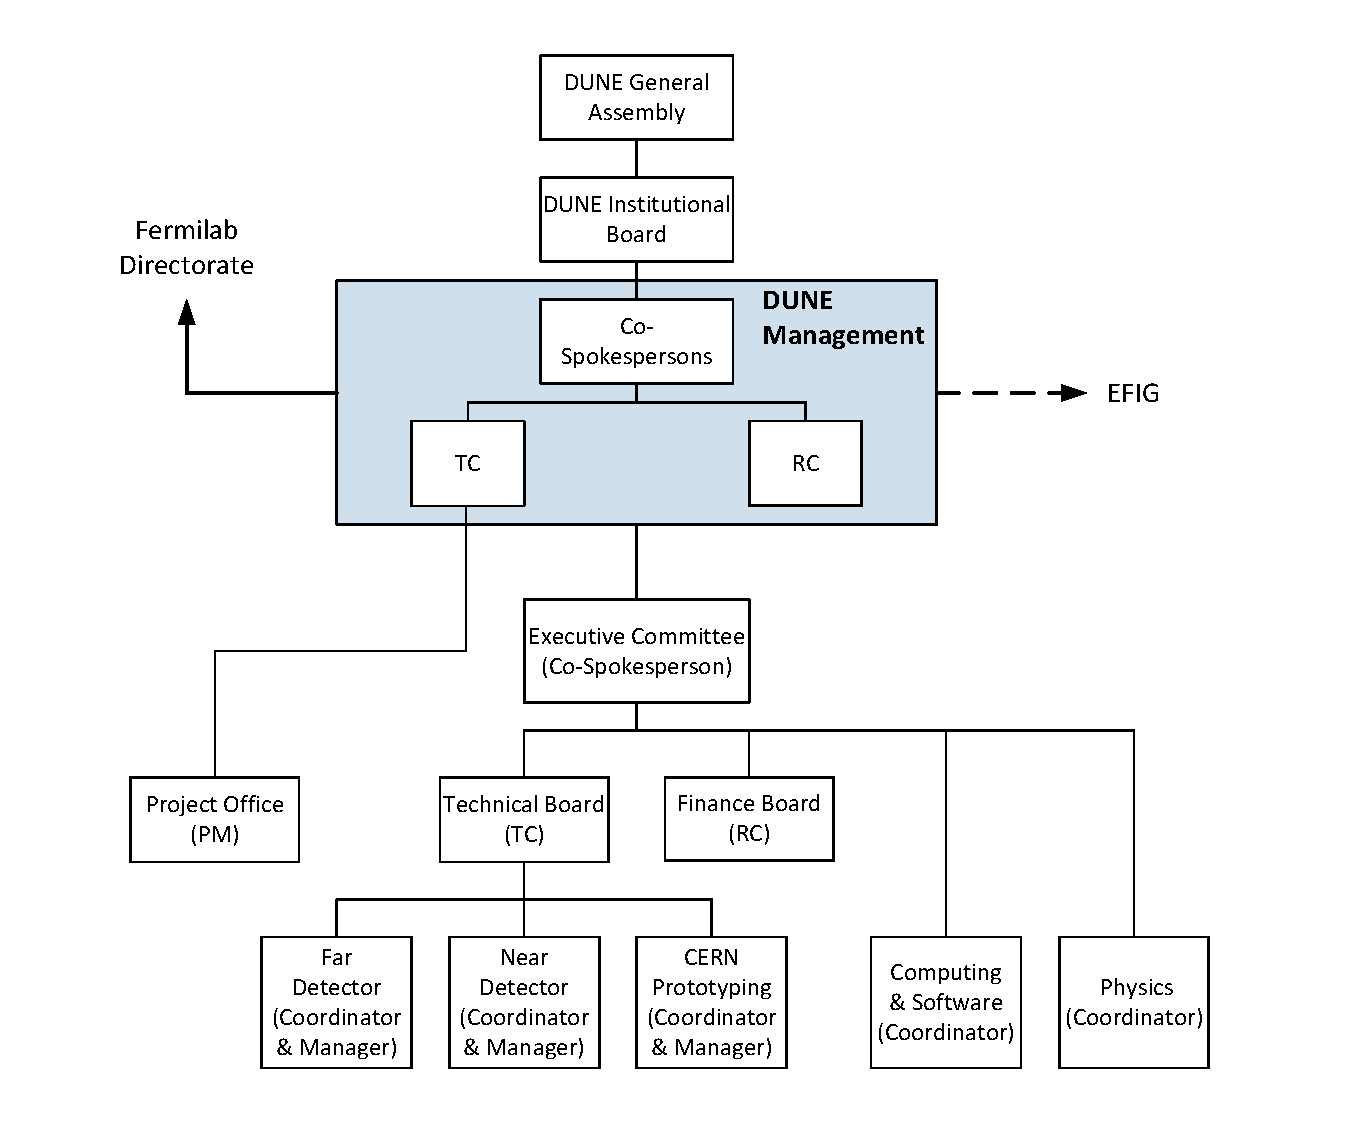
\includegraphics[width=0.95\textwidth]{dune-collaboration-org}
\end{cdrfigure}

%\fixme{(for Anne) command to keep figure from floating ...}
\begin{cdrfigure}[DUNE Work Breakdown Structure]{dune-wbs}{DUNE Work Breakdown Structure}
  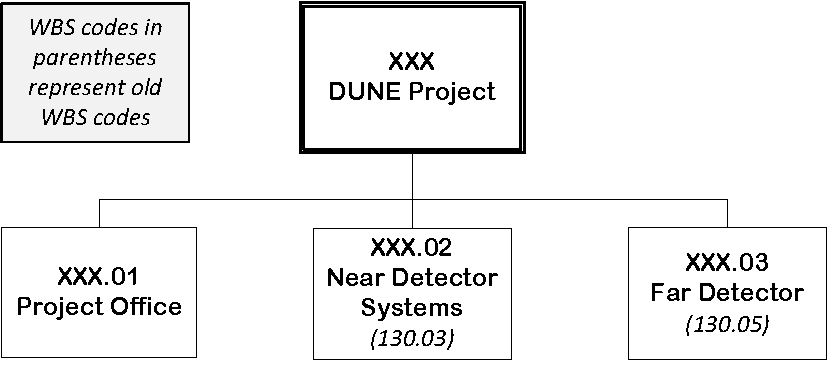
\includegraphics[width=0.8\textwidth]{dune-wbs-to-level3}
\end{cdrfigure}

%%%%%%%%%%%%%%%%%%%%%%%%%%%%%%
\subsection{DUNE Management Structure}

The main responsibilities of each of the roles are summarized below:
\begin{itemize}
 \item \textbf{DUNE General Assembly} is composed of the full membership of the Collaboration.  It is consulted on all major strategic decisions through open plenary sessions at Collaboration meetings and is provided regular updates on issues affecting the Collaboration at weekly Collaboration meetings.  The Collaboration General Assembly elects the co-spokespersons through a process defined by the Institutional Board.
\item \textbf{DUNE Institutional Board (IB)} is the representative body of the Collaboration institutions. It has responsibility for the governance of the Collaboration. The IB has final authority over Collaboration membership issues and defines the requirements for inclusion of individuals on the DUNE author list. The IB is also responsible for the process used to select the co-spokespersons and the Executive Committee.  The IB chairperson serves on the Executive Committee, runs the Institutional Board meetings, and organizes the Collaboration meetings.
\item \textbf{DUNE Co-Spokespersons} are elected by the Collaboration to serve as its leaders.  They direct Collaboration activities on a day-to-day basis and represent the Collaboration in interactions with the host laboratory, funding agencies, and the broader scientific community.
\item \textbf{DUNE Executive Committee (EC)} is the primary decision-making body of the Collaboration and is chaired by the longest serving Co-Spokesperson.  The membership of the EC consists of the Co-Spokespersons, the Technical Coordinator, the Resource Coordinator, the chair of the IB, and five additional members of the Collaboration (three elected IB representatives and two additional members selected by the Co-Spokespersons).  The EC operates as a decision-making body through consensus.  In cases where the EC is unable to reach a consensus, final decision-making authority is assigned to the Co-Spokespersons.  If the Co-Spokespersons are unable to reach their own consensus, the Fermilab Director will step in to resolve the issue.
\item \textbf{Technical Coordinator (TC)} is jointly appointed by the Co-Spokespersons and the Fermilab Director and has reporting responsibilities to both.  In the context of the international DUNE Project, the TC serves as the project director 
and is responsible for implementing the scientific and technical strategy of the Collaboration.  Currently, the TC also serves as project director for the DOE-funded portion of the DUNE Project.  In addition to managing the Project Office, the TC chairs the Collaboration Technical Board which coordinates activities associated with the design, construction, installation, and commissioning of the %different 
detector elements.
\item \textbf{Technical Board (TB)} is chaired by the TC and has a membership that includes the coordinators and managers of the Collaboration detector and prototyping groups.  It may also include additional members of the Collaboration, nominated by the TC and approved by the EC, who are expected to bring useful knowledge and expertise to its discussions on technical issues.  The TB is the primary %collaboration body where 
forum for discussion of issues related to %the 
detector design, construction, installation and commissioning. % are discussed.  
This body serves as a Project change-control board for change requests with schedule and cost impacts that lie below pre-determined thresholds necessitating EC approval.  Change requests that have impacts on interfaces with the LBNF Project, %potentially impact DUNE science requirements
potential impacts on DUNE science requirements, or that require modifications of formal Memoranda of Understanding (MOU) with one or more 
%funding agencies contributing to the project, 
contributing funding agencies, are discussed within the TB; however these require higher-level approvals, starting with the EC.  The TB is also the primary forum for discussing technological design choices faced by the Collaboration.  Based on these discussions, the TB is expected to make a recommendation on the preferred technology choice to the TC, who is then charged with making a final recommendation to the EC. %%%%%%%%%%%%%%%% Anne to here 5/26 2:30
\item \textbf{Resource Coordinator (RC)} is jointly appointed by the Co-Spokespersons and the Fermilab Director and has reporting responsibilities to both.  The RC chairs the Collaboration Finance Board and is tasked with preparing the formal MOUs that define the contributions and responsibilities of each institution.  The RC is also responsible for management of the common financial resources of the Collaboration (common fund).  Project change requests approved by the EC that involve modification of MOUs with one or more of the participating funding agencies are taken by the RC first to the Collaboration Finance Board for discussion and then, in cases where consensus is obtained, to the Resources Review Board for final approval.
\item \textbf{Finance Board (FB)} is chaired by the RC and has a membership that includes a single representative from each group of collaborating institutions whose financial support for participating in the DUNE experiment originates from a single, independent funding source.  These Collaboration representatives are either nominated through their respective group of institutions and approved by the associated funding agency, or directly appointed by the funding agency.  The FB discusses issues related to Collaboration resources such as contributions to Project common funds and division of Project responsibilities among the collaborating institutions.  The FB is also responsible for vetting proposed Project change requests prior to their submission to the Resource Research Board for approval.
\item \textbf{DUNE Science Coordinators} include the coordinators of the detector and prototyping groups as well as the coordinators of the DUNE physics and computing/software efforts.  Science coordinators are nominated by the Co-Spokespersons (jointly with the TC in the case of detector and prototyping group coordinators) and approved by the EC.  These coordinators are expected to establish additional Collaboration sub-structures within their assigned areas to cover the full scope of Collaboration activities within their areas of responsibility.  Detector and prototyping group coordinators report to the EC through the TB, while coordinators of the physics and software/computing efforts report directly to the EC.

\item \textbf{DUNE Project Office (PO)} provides the project management for the design, construction, installation, and commissioning of the DUNE near and far detectors.  Members of the Project Office, including the Project Manager (PM), are appointed by the  TC.  The DUNE Project will be run as an international project following DOE guidelines.  The PO will have control over common funds collected from the U.S. and international stakeholders.  Other contributions to the DUNE Project are expected to be in the form of deliverables as defined through formal MOUs. The PO will maintain a full schedule for the entire DUNE Project and track contributions through detailed subproject milestones.  The entire DUNE Project (including international contributions) will follow the DOE critical decision process incorporating a CD-2 approval of its baseline cost and schedule and a CD-3 approval for moving forward with construction.  The current high-level WBS structure of the DUNE Project, which will be evolving in the near future to best take advantage of the additional resources available within the new Collaboration, is illustrated in Figure~\ref{fig:dune-wbs}.

\item \textbf{DUNE Detector and Prototyping Managers} provide the required interface between the DUNE Project and the members of the Collaboration contributing to these efforts.  These managers sit within the detector and prototyping groups where all matters related to the design, construction, installation, and commissioning of the individual detector elements are discussed.  These managers are tasked with implementing the plans developed within their group and are part of a joint management team which addresses issues associated with Project interfaces and coordination of detector and prototyping group efforts.
\end{itemize}

%%%%%%%%%%%%%%%%%%%%%%%%%%%%%%%%%%%%%%%%%%%%%%%%%%%%%
\section{LBNF/DUNE Advisory and Coordinating Structures}
\label{sec:lbnf-dune-interface}

A set of structures is established to provide coordination among the participating funding agencies, oversight of the LBNF and DUNE projects, and coordination and communication between the two projects.  These structures and the relationships among them are shown in Figure~\ref{fig:lbnfdune-org} and described in this section

\begin{cdrfigure}[Joint LBNF/DUNE Management Structure]{lbnfdune-org}{Joint LBNF/DUNE Management Structure}
  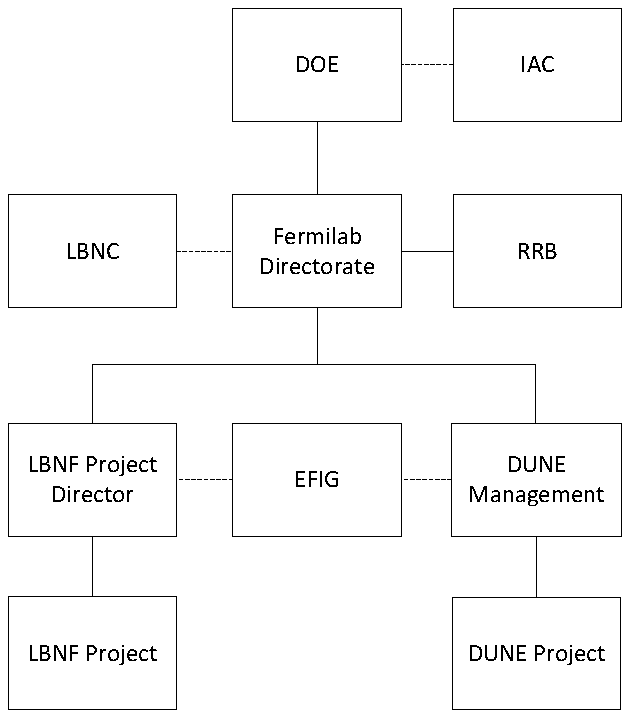
\includegraphics[width=0.8\textwidth]{joint-org}
\end{cdrfigure}


\subsection{International Advisory Council (IAC) }

The International Advisory Council (IAC) is composed of
regional representatives, such as CERN, and representatives of
funding agencies that make major contributions to LBNF infrastructure or to DUNE. The IAC 
acts as the highest-level international advisory body to the U.S.
DOE and the FNAL Directorate and facilitates
high-level global coordination across the entire enterprise (LBNF and DUNE).
The IAC is chaired by the DOE Office of Science Associate Director
for High Energy Physics and includes the FNAL Director in its membership.  
The council meets as needed and provides pertinent advice to 
LBNF and DUNE  
through the Fermilab Director.  


Specific responsibilities of the IAC include, but are not limited to,
the following:


\begin{itemize}
\item During the formative stages of LBNF and DUNE
the IAC helps to coordinate the sharing of responsibilities among
the agencies for the construction of LBNF and DUNE.
Individual agency responsibilities for LBNF will be established in
bilateral international agreements with the DOE. Agency contributions to
DUNE will be formalized through separate agreements.

\item The IAC assists in resolving issues, especially those
that cannot be resolved at the Resources Review Boards (RRB) level,
e.g., issues that require substantial redistributions of
responsibilities among the funding agencies.

\item The IAC assists as needed in the coordination,
synthesis and evaluation of input from Project reports charged by
individual funding agencies, LBNF and DUNE Project management,
and/or the IAC itself, leading to recommendations for action by
the managing bodies.
\end{itemize}

The initial membership, as of May 19, 2015, of the IAC is as follows:
James Siegrist (DOE HEP, Chair),
Sergio Bertolucci (CERN),
Arun Srivastava (DAE),
Carlos Henrique de Brito Cruz (FAPESP),
Fernando Ferroni (INFN),
Fabiola Gianotti (CERN),
Rolf Heuer (CERN),
Stavros Katsanevas (ApPEC),
Frank Linde (ApPEC),
Nigel Lockyer (FNAL),
Reynald Pain (IN2P3/CNRS),
John Womersley (STFC) and
Agnieszka Zalewska (IFJ).

The DUNE Co-Spokespersons and/or other participants within
the Fermilab neutrino program will be invited to sessions of the IAC as
needed. Council membership may increase as additional funding agencies
from certain geographic regions make major contributions to LBNF and DUNE.

\subsection{Resources Review Boards (RRB)}

The Resources Review Boards (RRB) are composed of representatives of all
funding agencies that sponsor LBNF and DUNE, and of the Fermilab
management. The RRB provides focused monitoring and detailed oversight
of each of the Projects. The Fermilab Director in coordination
with the DUNE RC defines its membership. A representative from the
Fermilab Directorate chairs the boards and
organize regular meetings to ensure the flow of resources needed
for the smooth progress of the enterprise 
and for its successful completion.  
The managements of the
DUNE Collaboration and the LBNF Project participates in the RRB meetings
and make regular reports to the RRB on technical, managerial,
financial and administrative matters, as well as status and
progress of the DUNE Collaboration.

There are two groups  
within the RRB: RRB-LBNF and RRB-DUNE. Each of
these groups monitors progress and addresses 
 the issues specific to its area 
 while the whole RRB deals with matters
that concern the entire enterprise. 
The RRB will meet
biannually; these meetings 
will start with a plenary
opening session 
and be followed by 
RRB-LBNF and RRB-DUNE sessions. As DUNE progresses toward
experimental operations, RRB-Computing sessions will convene.

DUNE Finance Board members who serve as National Contacts from the 
sponsoring funding agencies will be invited to RRB sessions.

The RRB  employs standing DUNE and LBNF \textit{Scrutiny Groups} as needed
to assist in its responsibilities. The scrutiny groups operate
under the RRB, and provide detailed information on financial and
personnel resources, costing, and other elements under the purview of the RRB.

Roles of the RRB includes:

\begin{itemize}
\item assisting the DOE and the FNAL Directorate,
with coordinating and developing any required international
agreements between partners
\item monitoring and overseeing the Common Projects and the
use of the Common Funds
\item monitoring and overseeing general financial and personnel support
\item assisting the DOE and the FNAL Directorate
with resolving issues that may require reallocation of responsibilities
among the Project's funding agencies
\item reaching consensus on a maintenance and operation procedure,
and monitoring its function
\item  approving the annual construction, and maintenance and operation common fund 
budget of DUNE
\end{itemize}

\subsection{Fermilab, the Host Laboratory}

As the host laboratory, Fermilab has a direct responsibility for the design,
construction, commissioning and operation of the facilities and
infrastructure (LBNF) that support the science program. 
In this capacity, Fermilab reports
directly to the DOE through the Fermilab Site Office (FSO).
Fermilab also has an important oversight role for the DUNE Project
itself as well as an important coordination role in ensuring that
interface issues between the two Projects are completely understood.

Fermilab's oversight of the DUNE Collaboration and detector
construction project is carried out through
\begin{itemize}
\item regular meetings with the Collaboration leadership
\item approving the selection of Collaboration spokespersons
\item  providing the Technical and Resource Coordinators
\item  convening and chairing the Resources Review Boards
\item  regular scientific reviews by the PAC and LBNC
\item  Director's Reviews of specific management, technical,
cost and schedule aspects of the detector construction project
\item other reviews as needed
\end{itemize}

\subsection{DUNE Collaboration}	

The Collaboration, in consultation with the Fermilab Director,
is responsible for forming the international DUNE Project team 
responsible for designing and constructing the detectors.  
The Technical Coordinator
(TC) and Resource Coordinator (RC) serve as the lead managers
of this international project team and are selected jointly by
the spokespersons and the Fermilab Director.  Because the international DUNE
Project incorporates contributions from a number of different
funding agencies, it %the international DUNE project 
is responsible for
satisfying individual tracking and reporting requirements associated
with %each of 
the different contributions.

\subsection{Long-Baseline Neutrino Committee (LBNC)}

The Long-Baseline Neutrino Committee (LBNC), composed
of internationally prominent scientists with relevant expertise,
provides external scientific peer review for LBNF and DUNE %two projects 
regularly.
The LBNC reviews the scientific, technical and managerial
decisions and preparations for the neutrino program.
It acts in effect %effectively 
as an adjunct to the Fermilab Physics Advisory Committee
(PAC), meeting on a more frequent basis than the PAC.
The LBNC may employ DUNE and LBNF Scrutiny Groups for more
detailed reports and evaluations. The LBNC members are appointed by the
Fermilab Director. The current membership of the LBNC is:
%
David MacFarlane (SLAC, Chair),
Ursula Bassler (IN2P3),
Francesca Di Lodovico (Queen Mary),
Patrick Huber (Virginia Tech),
Mike Lindgren (FNAL),
Naba Mondal (TIFR),
Tsuyoshi Nakaya (Kyoto),
Dave Nygren (UT Arlington),
Stephen Pordes (FNAL),
Kem Robinson (LBNL),
Nigel Smith (SNOLAB) and
Dave Wark (Oxford and STFC).
%
Among these members, David McFarlane and Dave Wark are also members of the Fermilab PAC.

\subsection{Experiment-Facility Interface Group (EFIG)}

Close and continuous coordination between DUNE and LBNF is
required to ensure the success of the combined enterprise.
An Experiment-Facility Interface Group (EFIG) was established
in January 2015 to oversee and ensure the required coordination
both during the design/construction and operational
phases of the program. This group covers areas including:
\begin{itemize}
\item  interface between the near and far detectors and the
corresponding conventional facilities
\item interface between the detector systems provided by
DUNE and the technical infrastructure provided by LBNF
\item design and operation of the LBNF neutrino beamline
\end{itemize}

The EFIG is chaired by two deputy directors of Fermilab.
Its membership includes the LBNF Project Director, Project Manager and Project Scientist, and 
the DUNE Co-Spokespersons, Technical Coordinator, Resource Coordinator and the CERN-LBNF Project Manager.
In consultation with the DUNE and LBNF management, the EFIG Chairs will
extend the membership as needed 
to carry out the coordination
function. In addition, the DOE Federal Project Director for LBNF,
the Fermilab Chief Project Officer, and a designated representative
of the South Dakota Science and Technology Authority (SDSTA) will
serve ex officio. The EFIG Chairs designate a Secretary of the EFIG,
who keeps minutes of the meetings and performs other tasks as
requested by the Chair.

It is the responsibility of the EFIG Chairs to report EFIG proceedings
to the Fermilab Director and other stakeholders. It is the responsibility
of the DUNE spokespersons to report EFIG proceedings to the rest of
the Collaboration. The EFIG meets weekly or as needed.

The current membership of the EFIG is:
%
Joe Lykken (representing Fermilab Director, Chair),
Nigel Lockyer (acting LBNF Project Director),
Elaine McCluskey (LBNF Project Manager),
Jim Strait (LBNF Project Scientist),
\hyphenation{Andr\'e}
Andr\'e Rubbia (DUNE co-spokesperson),
Mark Thomson (DUNE co-spokesperson),
Eric James (DUNE Technical Coordinator),
Chang Kee Jung (DUNE Resource Coordinator),
Marzio Nessi (CERN),
David Lissauer (BNL),
Jim Stewart (BNL),
Jeff Dolph (BNL, Secretary),
Mike Lindgren (FNAL Chief Project Officer, ex officio),
Pepin Carolan (DOE, ex officio), and 
Mike Headley (SDSTA, ex officio).


